
%!TEX ROOT=ctutest.tex

\chapter{Odvozené parametry}

Identifikované parametry jsou uvedeny v tabulce \ref{tab_ind_hodnot}. Křížkem jsou označeny hodnoty, které se nepodařilo plně identifikovat. Hodnoty jsou uvedeny v základních jednotkách SI. Z tabulky je možné vypozorovat, že šestý link se podařilo identifikovat plně. Problém nastal už u linku č.5, jehož hmotnost vyšla nulová, protože neměla při těchto průbězích na dynamiku vliv. Kvůli tomu již hmotnosti následujících linků nemohou být správně identifikovány, protože jejich rovnice jsou na tomto parametru závislé.  
\\

\begin{table}[htbp]
  \centering
  \caption{Tabulka odvozených parametrů}
    \begin{tabular}{c|cccccccccc}
    \multicolumn{1}{c|}{Osa} & \multicolumn{1}{c}{$I_{xx}$} & \multicolumn{1}{c}{$I_{yy}$} & \multicolumn{1}{c}{$I_{zz}$} & \multicolumn{1}{c}{$d_x$} & \multicolumn{1}{c}{$d_y$} & \multicolumn{1}{c}{$d_z$} & \multicolumn{1}{c}{$m$} & \multicolumn{1}{c}{$f_v$} & \multicolumn{1}{c}{$f_c$} \\
    \hline
    1     &        &        &  x     &   x    &  x     &  x     &   x    &   x    & x \\
    2     &   x    &  x     &  x     &   x    &  x     &  x     &   x    &  x     & x \\
    3     &   x    & x      &   x    &   x    &   x    &    x   &   x    &  x     &  x\\
    4     &   0    &  0     & 0.013 & 0.0053 & -0.001 &   x    &   0    & 0.1516 &  0.2757\\
    5     & 0     & 0.013 & 0.0135 & -0.0017 & 0.007 & 0.001 & 0     & 0.0739 & 0.1576 \\
    6     & 0.0065 & 0.007 & 0.0049 & -0.0047 & -0.0012 & -0.0039 & 0.0055 & 0.0835 & 0.1926 \\
    \end{tabular}%
  \label{tab_ind_hodnot}%
\end{table}%

\newpage 

\section{Simulace odvozených parametrů}

Na následujících obrázcích jsou odsimulované točivé momenty s odvozenými parametry pro osy 4 až 6. Pro další osy simulace provedeny nebyly, protože se pro ně nepodařilo správně odvodit všechny jejich dynamické parametry.

Na obrázku \ref{osa6_prub_a} je porovnání mezi skutečným naměřeným momentem a vypočítaným z odvozených parametrů pro osu 6. Na druhém obrázku \ref{osa6_prub_b} je poté zobrazena okamžitá a průměrná odchylka mezi naměřeným a vypočítaným momentem. 

\begin{figure}[!h]
  \centering
  \subfloat[Srovnání naměřených a vypočítaných momentů]{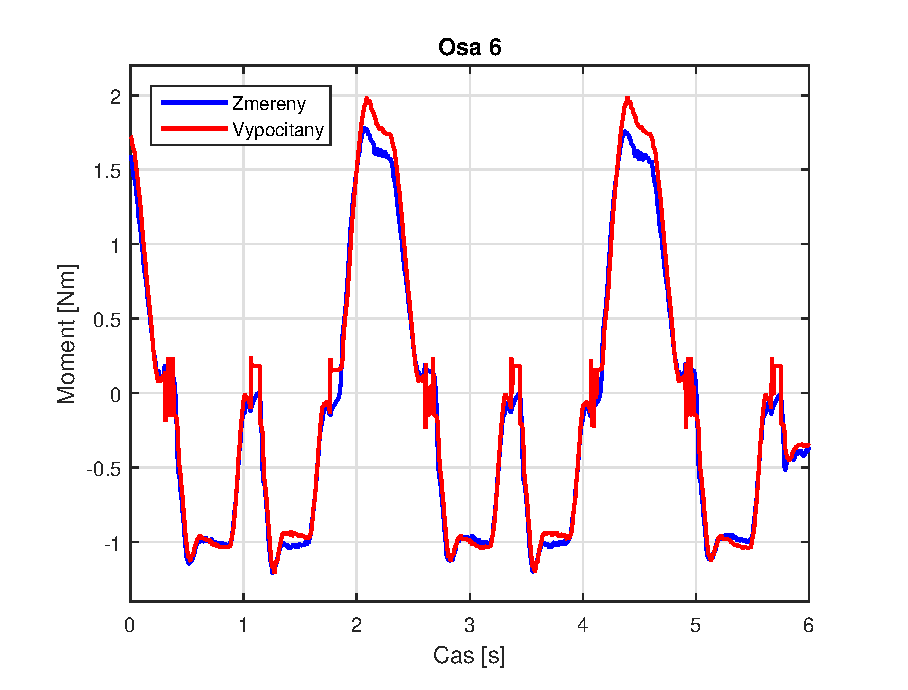
\includegraphics[width=0.5\textwidth]{Osa_6}\label{osa6_prub_a}}
  \hfill
  \subfloat[Okamžitá a průměrná odchylka]{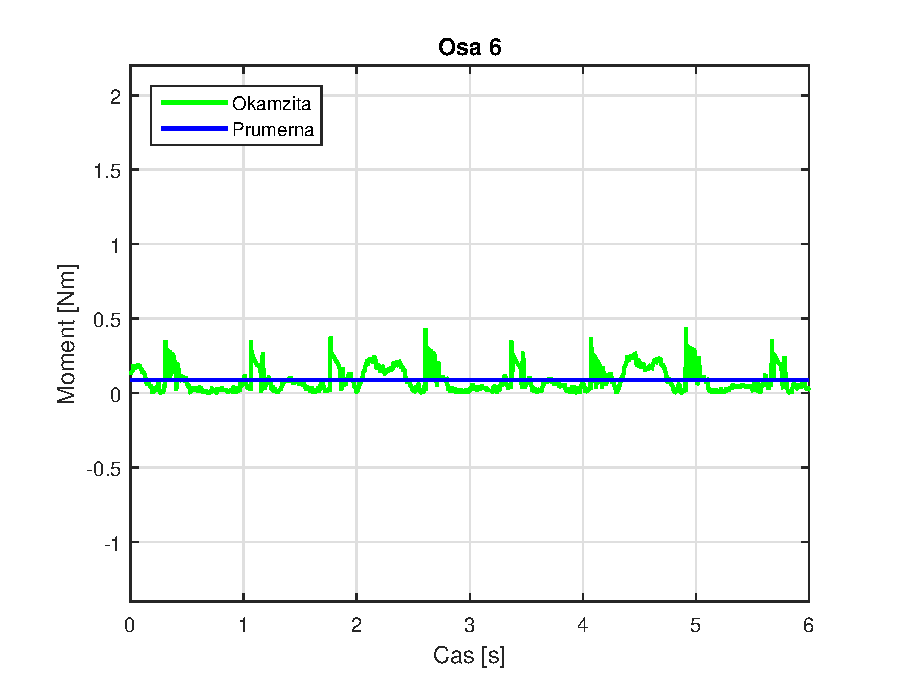
\includegraphics[width=0.5\textwidth]{Osa_6_odch}\label{osa6_prub_b}}
  \caption{Točivé momenty pro osu 6.}
  \label{osa6_prub}
\end{figure}

Stejné průběhy pro osu 5 jsou na obrázku \ref{osa5_prub} a pro osu 4 na obr. \ref{osa4_prub}.

\begin{figure}[!h]
  \centering
  \subfloat[Srovnání naměřených a vypočítaných momentů]{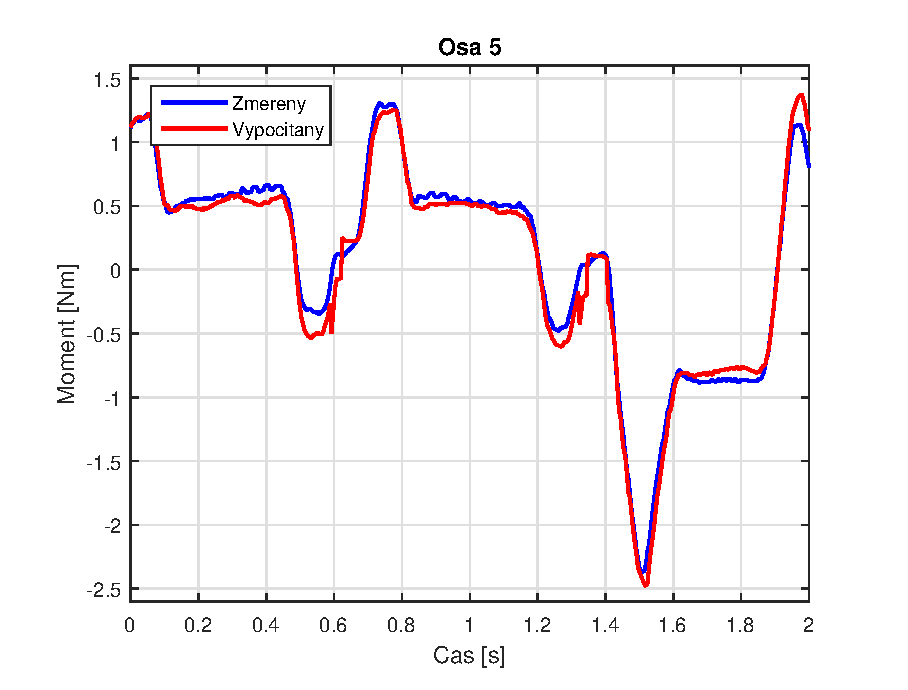
\includegraphics[width=0.5\textwidth]{Osa_5}\label{osa5_prub_a}}
  \hfill
  \subfloat[Okamžitá a průměrná odchylka]{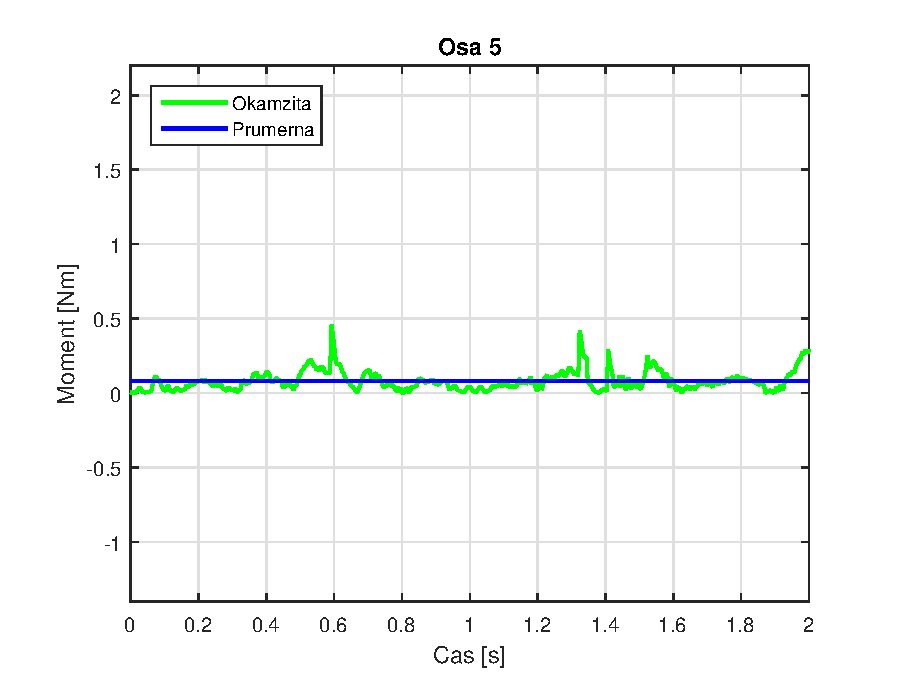
\includegraphics[width=0.5\textwidth]{Osa_5_odch}\label{osa5_prub_b}}
  \caption{Točivé momenty pro osu 5.}
  \label{osa5_prub}
\end{figure}
\newpage

\begin{figure}[!h]
  \centering
  \subfloat[Srovnání naměřených a vypočítaných momentů]{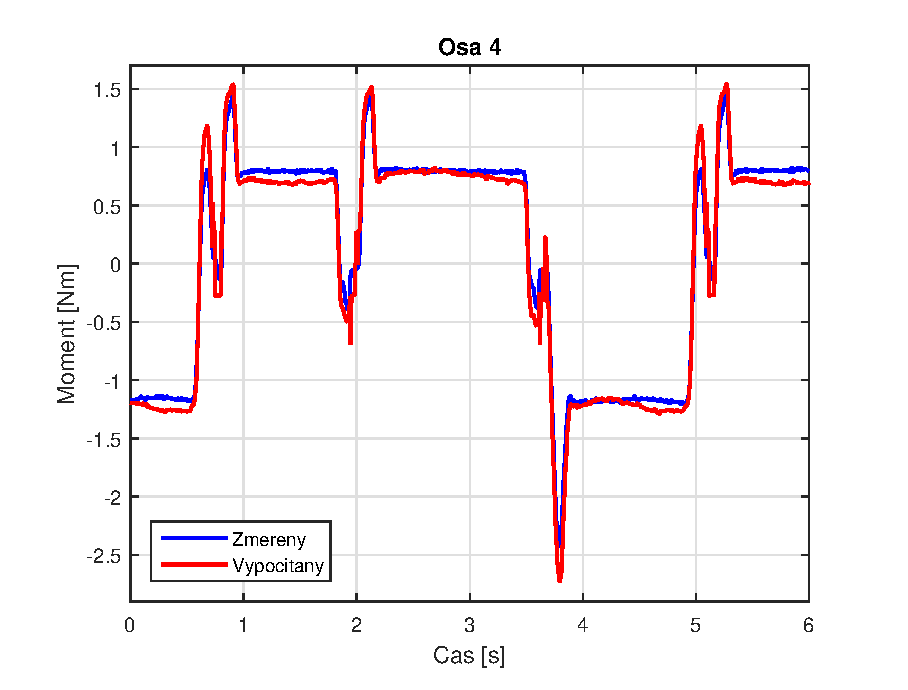
\includegraphics[width=0.5\textwidth]{Osa_4}\label{osa4_prub_a}}
  \hfill
  \subfloat[Okamžitá a průměrná odchylka]{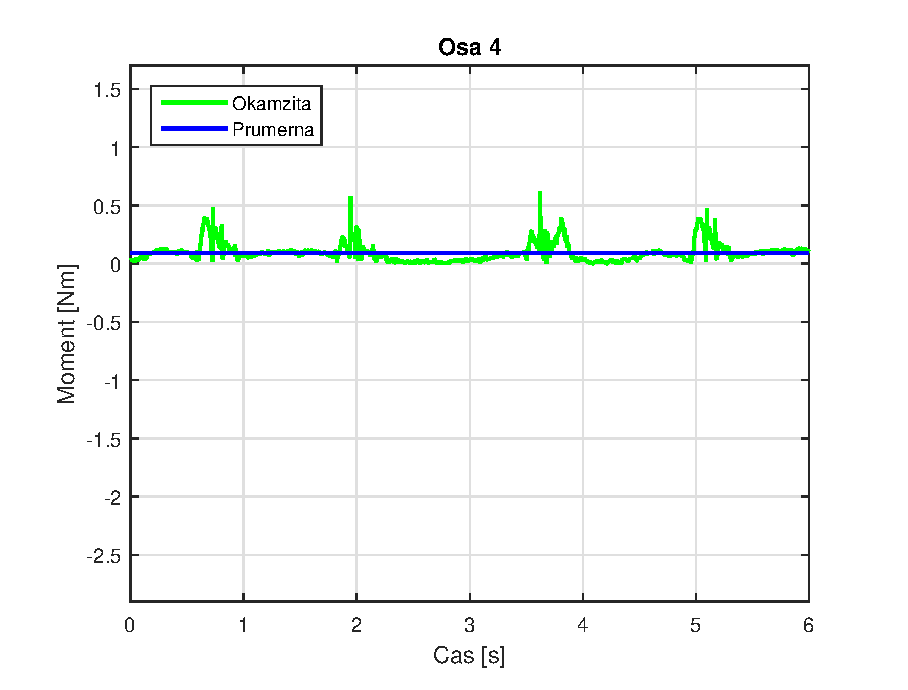
\includegraphics[width=0.5\textwidth]{Osa_4_odch}\label{osa4_prub_b}}
  \caption{Točivé momenty pro osu 4.}
  \label{osa4_prub}
\end{figure}

Z výše uvedených průběhů je patrné, že vypočítané a naměření průběhy si poměrně odpovídají. Ve všech případech se průměrná odchylka pohybuje kolem jedné desetiny Nm a maximální okamžitá odchylka nepřesahuje šest desetin Nm. 

 